\documentclass[twoside,10pt,a4paper]{article}
\usepackage[utf8]{inputenc}
\usepackage[english]{babel}
\usepackage{amsmath}
\usepackage{amsfonts}
\usepackage{amssymb}
\usepackage{graphicx}

\usepackage[left=2cm,right=2cm,top=2cm,bottom=3cm]{geometry}
\usepackage{fancyvrb}
\usepackage{listings}
\usepackage{xparse}
\usepackage{tikz} % ajout de dessins LaTeX
\usepackage{graphicx}
\usepackage{float}  % alignement des figures
\usepackage{fancyhdr}
\usepackage{enumitem}
\usepackage{verbatim}
\usepackage{xcolor}

\usepackage{caption}
\usepackage{subcaption}

\pagestyle{fancy} %fancyhdr
	\fancyhf{} %fancyhdr
	\renewcommand{\sectionmark}[1]{\markboth{#1}{}}
	\fancyhead[R]{NLDCI Set 6 Questions} %INSERT TITLE HERE FOR fancyhdr
	\fancyhead[L]{\nouppercase{\leftmark}} %fancyhdr
	\cfoot{\thepage} %fancyhdr
	\setlength{\headheight}{35pt}
	\setlength{\parindent}{0pt}
	
	\definecolor{MyBlue}{HTML}{4A90E2}
	\definecolor{MyRed}{HTML}{D0021B}
	\definecolor{MyGreen}{HTML}{7ED321} % Same color use in Mathcha

\begin{titlepage}
\title{\huge \textbf{Nonlinear Dynamics \& Chaos I \\ \Large Exercice Set 6 Questions}}	%TITLE
\author{ }		%AUTHOR
\date{ }	%DATE

\end{titlepage}


\begin{document}

\maketitle

\section*{Question 1}
Which quantity is conserved along the trajectories of $\ddot{x} - x + x^3 = 0$?

\begin{enumerate}[label=(\alph*)]
	\item $ \displaystyle  H(x, \dot{x}) = \dot{x}^2 - x^2 + \frac{1}{4}x^4 $
	\item $ \displaystyle  H(x, \dot{x}) = \dot{x}^2 - x^2 + \frac{1}{8}x^4 $
	\item $ \displaystyle  H(x, \dot{x}) = \frac{1}{2}\dot{x}^2 - \frac{1}{2}x^2 + \frac{1}{4}x^3 $
	\item $ \displaystyle  H(x, \dot{x}) = \dot{x}^2 - x^2 + \frac{1}{2}x^4 $
\end{enumerate}

\section*{Question 2}
Consider the dynamical system
\begin{equation*}
	\begin{cases}
		\dot{x} = y + f(x,y) \\
		\dot{y} = x + g(x,y)
	\end{cases}
\end{equation*}
Where $x,y \in \mathbb{R}$. Which condition is \underline{sufficient} for this dynamical system \underline{not} to have a limit cycle?

\begin{enumerate}[label=(\alph*)]
	\item $ \displaystyle f(x,y)g(x,y) < 0, \quad \forall x,y $
	\item $ \displaystyle \frac{\partial f}{\partial y} - \frac{\partial g}{\partial x} < 0, \quad \forall x,y $
	\item $ \displaystyle \frac{\partial f}{\partial x} + \frac{\partial g}{\partial y} < 0, \quad \forall x,y $
	\item None of the above
\end{enumerate}

\section*{Question 3}
Consider the system
\begin{equation*}
	\begin{cases}
		\dot{r} = r(1 - r) \\
		\dot{\theta} = \sin^2 \left( \frac{\theta}{2} \right)
	\end{cases}
\end{equation*}
written in polar coordinates $(r, \theta)$. With the phase portrait depicted in the figure below, which statement is correct ?

\begin{figure}[H]
	\centering
	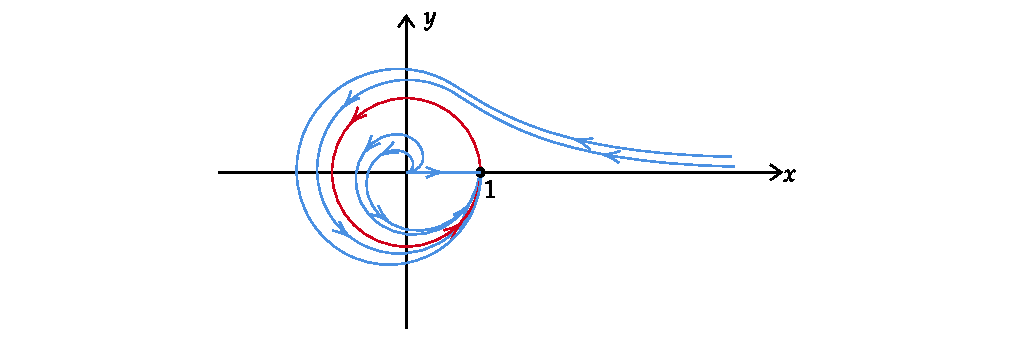
\includegraphics[scale=0.9]{Graphics/MCQ1_figures/Q16D01.pdf}
	\caption{Phase portrait of the system.}
\end{figure}

\begin{enumerate}[label=(\alph*)]
	\item The fixed point $(x = 0, y = 0)$ is the $\alpha$-limit point for any $(x_0, y_0)$.
	\item The fixed point $(x = 1, y = 0)$ is asymptotically stable.
	\item The fixed point $(x = 1, y = 0)$ is the $\omega$-limit point for any $(x_0, y_0) \neq (0,0)$.
	\item The invariant curve $r=1$ is the $\omega$-limit point for any $(x_0, y_0)$ with $x^2 + y^2 = 1$.
\end{enumerate}

\section*{Question 4}
The phase portrait of four dynamical systems are depicted below. Which phase portrait is robust under small enough perturbations?

\begin{enumerate}[label=(\alph*)]
	\item 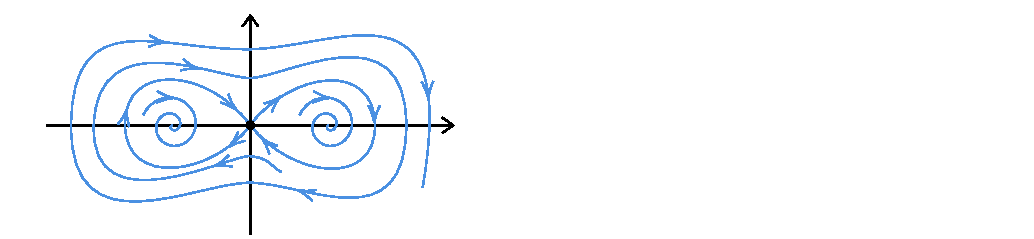
\includegraphics[scale=0.8]{Graphics/MCQ1_figures/Q18D01.pdf}
	\item 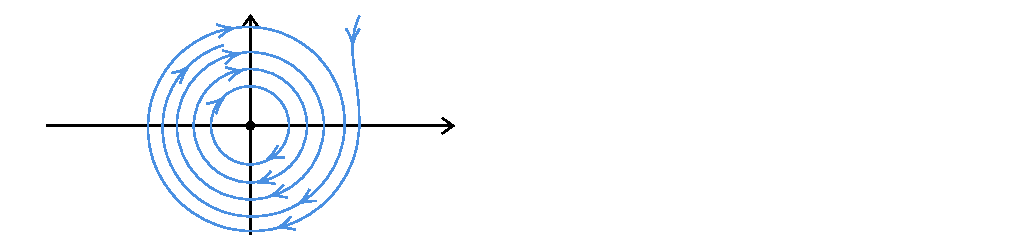
\includegraphics[scale=0.8]{Graphics/MCQ1_figures/Q18D02.pdf}
	\item 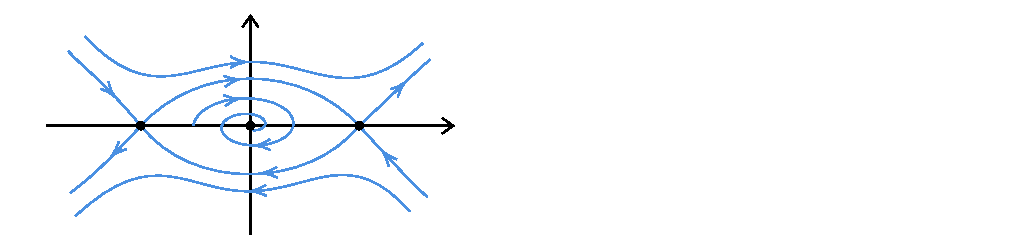
\includegraphics[scale=0.8]{Graphics/MCQ1_figures/Q18D03.pdf}
	\item 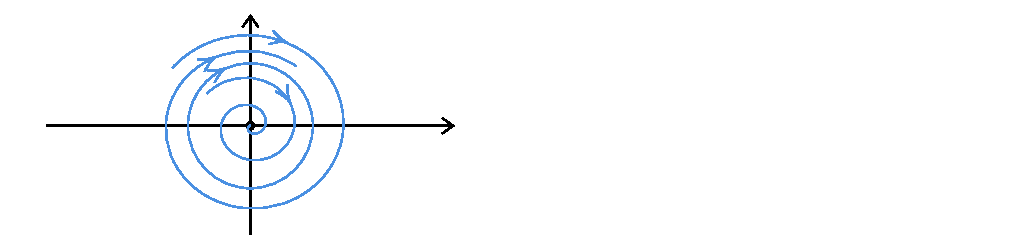
\includegraphics[scale=0.8]{Graphics/MCQ1_figures/Q18D04.pdf}
\end{enumerate}

\section*{Question 5}
A one-degree-of-freedom mechanical system has a first integral
\begin{equation*}
	E(x, \dot{x}) = \frac{1}{2}\dot{x}^2 + V(x)
\end{equation*}
where the graph of $V(x)$ is shown below. Which figure may correspond to the phase portrait of the mechanical system?

\begin{figure}[H]
	\centering
	
\includegraphics[scale=0.9]{Graphics/MCQ1_figures/Q21D01.pdf}
	\caption{Potential function $ V(x) $ of the mechanical system.}
\end{figure}

\begin{enumerate}[label=(\alph*)]
	\item 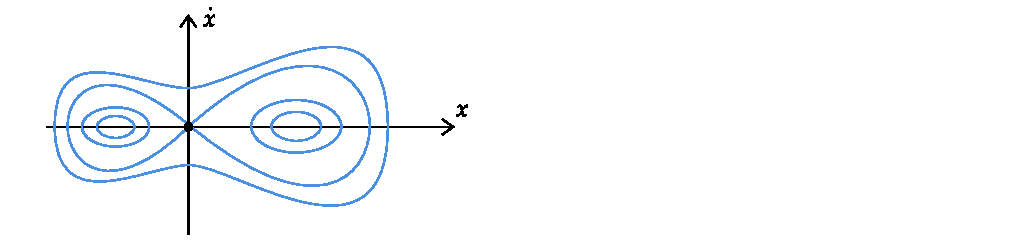
\includegraphics[scale=0.8]{Graphics/MCQ1_figures/Q21D02.pdf}
	\item 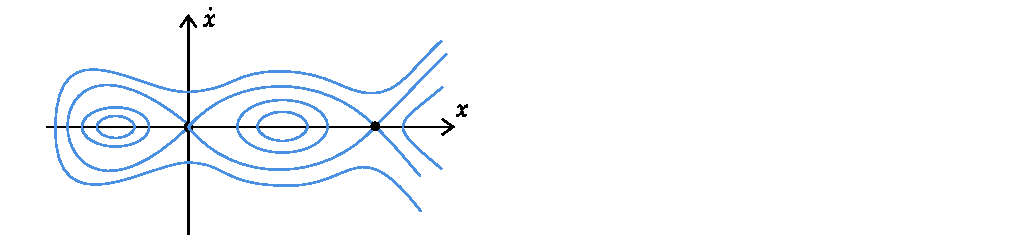
\includegraphics[scale=0.8]{Graphics/MCQ1_figures/Q21D03.pdf}
	\item 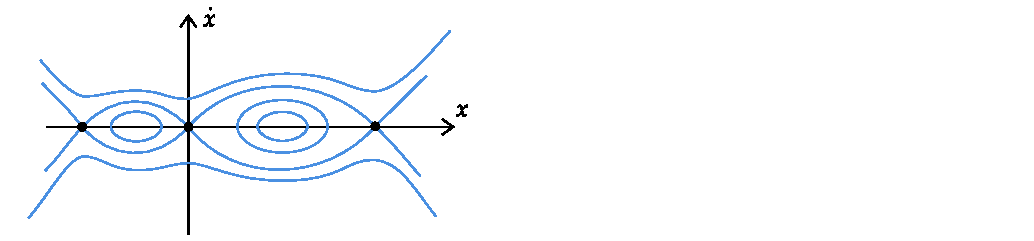
\includegraphics[scale=0.8]{Graphics/MCQ1_figures/Q21D04.pdf}
	\item 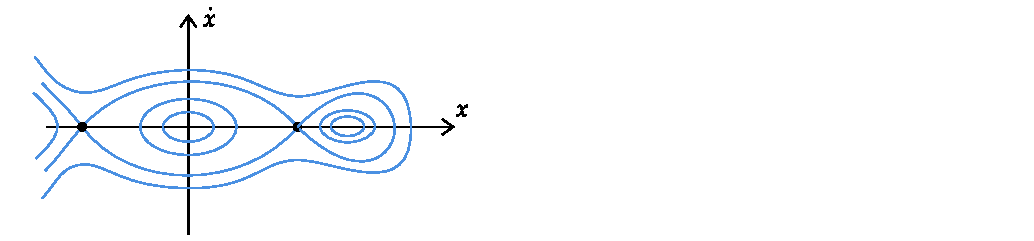
\includegraphics[scale=0.8]{Graphics/MCQ1_figures/Q21D05.pdf}
\end{enumerate}

\section*{Question 6}
Consider a planar dynamical system with the following phase portrait:

\begin{figure}[H]
	\centering
	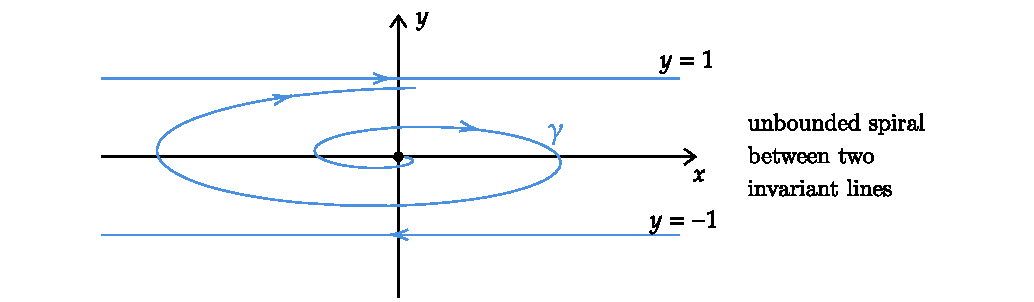
\includegraphics[scale=0.9]{Graphics/MCQ2_figures/Q04D01.pdf}
	\caption{Phase portrait of the planar dynamical system}
\end{figure}

Which of the following statement is true?

\begin{enumerate}[label=(\alph*)]
	\item The $\omega$-limit set of $\gamma$ is empty.
	\item By the Poincaré-Bendixson theorem, the $\omega$-limit set of $\gamma$ is composed of the lines $y = 1$ and $y = -1$.
	\item The Poincaré-Bendixson theorem does not apply to $\gamma$.
	\item None of the above
\end{enumerate}

\section*{Question 7}
Consider the Van der Pol equation
\begin{equation*}
	\ddot{x} + \alpha(x^2 - 1)\dot{x} + x = 0, \quad \alpha > 0, \quad x \in \mathbb{R}
\end{equation*}
Which of the following statements are true?

\begin{enumerate}[label=(\alph*)]
	\item This equation cannot have limit cycles.
	\item Any limit cycle of this equation must intersect at least one of the two lines $\{ x = 1 \}$, $\{ x = -1 \}$.
	\item Any limit cycles of this equation is necessarily unstable.
	\item None of the above
\end{enumerate}

\section*{Question 8}
Consider a particle sliding frictionlessly on the following terrain:

\begin{figure}[H]
	\centering
	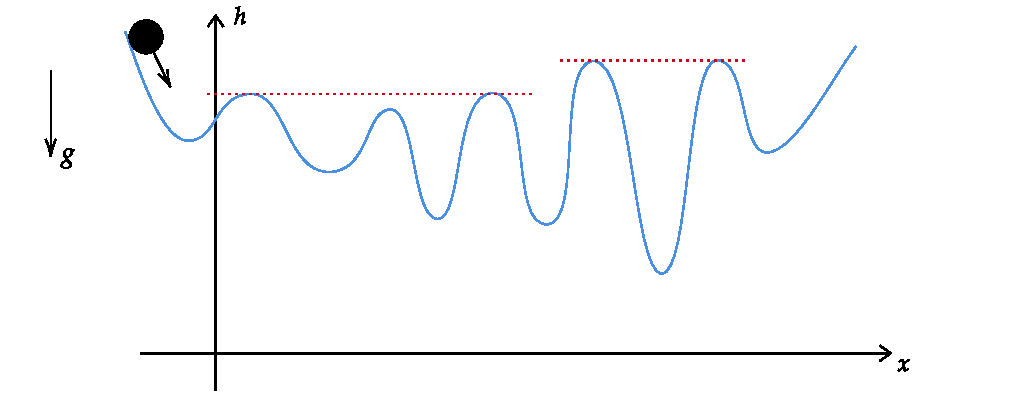
\includegraphics[scale=0.9]{Graphics/MCQ2_figures/Q09D01.pdf}
	\caption{Terrain on which the particle slides}
\end{figure}

Which of the following statements are true?

\begin{enumerate}[label=(\alph*)]
	\item The phase portrait of the dynamical system describing the motion of this particle cannot be drawn, as the available information is insufficient.
	\item A qualitative sketch of the phase protait is as follows:
	
	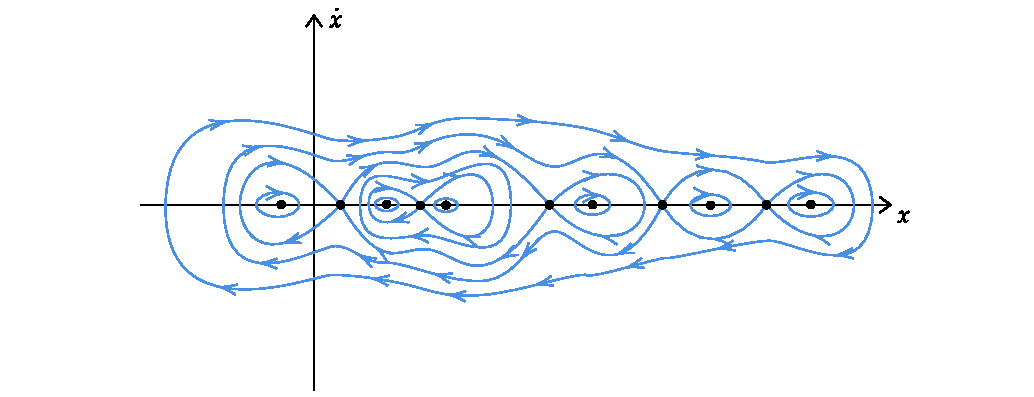
\includegraphics[scale=0.8]{Graphics/MCQ2_figures/Q09D02.pdf}
	\item A qualitative sketch of the phase portrait is as follows:
	
	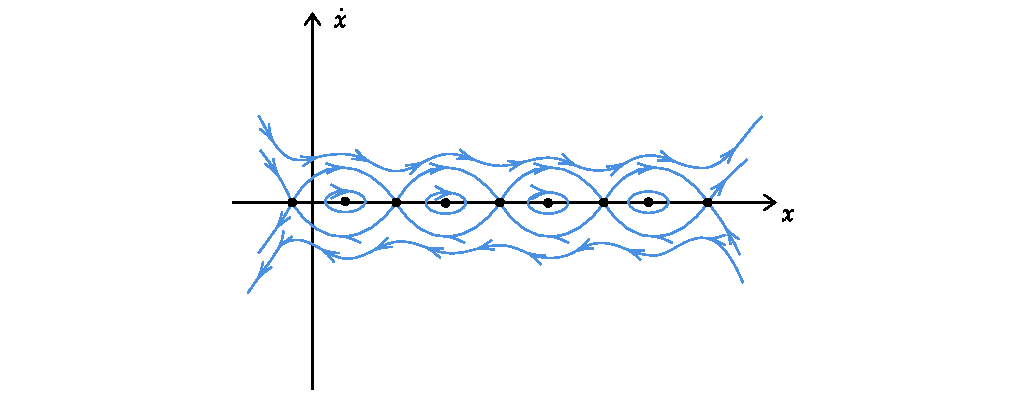
\includegraphics[scale=0.8]{Graphics/MCQ2_figures/Q09D03.pdf}
	\item This dynamical system must have at least one attracting limit cycle.
\end{enumerate}





\end{document}